\chapter{Tutorial}

In this capter we will walk you through basic manipulations of nucleic
datasets, tree building, naming conventions and overall usage to get
you started with \emph{MNHN-Tools}.

\section{Preparing your data}

At first let us get started with a dataset that you might have. For this
tutorial we recommand you to have a dataset of reasonable size at
hand. While these tools work and have been tested for millions of
sequences we recommand you that you use a dataset of about 5000 to
10000 sequences for this tutorial to progress fast and learn how to
use these tools quickly. If you have no dataset available you can
generate one with our built in virtual biosphere generator the
\emph{virtual\_evolution} tools shown in section
\ref{sec-virtual-ev}. To generate such a dataset you might run:
\lstset{language=bash,
  caption={Generate a test dataset using the \emph{virtual\_evolution}
  tools},
  label=lst-virtev-tutorial}
\begin{lstlisting}
virtual_evolution_controlled  15 100 10000 2 -1 50000 5 test.fasta
\end{lstlisting}
which should yield a decent dataset to discover \emph{MNHN-tools}.

The tools presented herein are built with FASTA \cite{fasta} files in mind. If
you have your sequence data available in a different file format you
may need to convert it beforehand. If you bring your own FASTA file
for this tutorial please note that the \emph{MNHN-tools} are only able
to treat human readable non single line FASTA files. 
As such a sequence may not contain more than 1000 characters per line.
If your file contains lines that are longer then the 1000 character
limit you may convert it to
a conforming FASTA file using the \emph{seqret} tool from EMBOSS
\cite{emboss}.
Several application domains of \emph{MNHN-Tools} are used to use FASTQ files.
If you have datasets in this format you may use the following
\emph{bash} script to convert your FASTQ files to FASTA files. 
\lstset{language=bash,
  caption={Script to convert FASTQ to FASTA files},
  label=lst-fastq2fasta}
\begin{lstlisting}
#!/bin/bash

sed -n '1~4s/^@/>/p;2~4p' $1 > $2
\end{lstlisting}
In such a case it might also be necessary to apply \emph{seqret} from
EMBOSS on the FASTA files resulting from this conversion in order to
ensur appropriate line lengths. 

Before using a dataset with \emph{MNHN-Tools} you further may make
sure that it is suited for the task that you would like to
achieve. The tools presented herein are in general made to
compare sequences of at least a reasonable similarity. As calculating
the consenus of unaligned datasets consisting of millions of
sequences might be cumbersum, we suggest to
examine the variation in sequence lengths first. The
\emph{lengths\_from\_fasta} tool is perfect for this task (c.f. section
\ref{sec-lengthsfromfasta}) and may be run like:
\lstset{language=bash,
  caption={\emph{lengths\_from\_fasta} tutorial},
  label=lst-lengthsfromfasta-tutorial}
\begin{lstlisting}
lengths_from_fasta your.fasta > lengths
\end{lstlisting}
The tool yields all the sequence lengths for the sequences of your
dataset on seperated lines in the \emph{lengths} file. We leave it to
the reader to analyze with the divers tools available to find out weather
the lenghts do not have a variance that is reasonable in resepect to
the average sequence length. 

\section{Investigating k-mers and Principal Components}

A convinient way to transform a set of sequences into an alignment
free representation, hence a representation where we do not need to
align sequences in order to calculate their distance or compare them
is the \emph{k-mer} representation. In the \emph{k-mer}
representation we compare all possibilties of sequences of certain $k$
length with a sequence in questions and count how often such a
sequence appears in our sequence of question. Let us image that $k$ equals
four. In such a case we obtain 256 possibilties to form a sequence ( out of
nucleotides ) or $4^4$ sequences. As we count how often any of these
sequences occurs in our target sequence, we can represent the target
sequence as a vector of 256 k-mer frequencies, a vector holding the
counts how often each sequence occurs in the target sequence for the
256 k-mers.
In order to perform this transformation we run the
\emph{fasta2kmer} tool (c.f. section \ref{sec-fasta2kmer}). In our case
we are not generating 4-mers, but 5-mers for our sequencies and thus
vectors of $5^{4}=1024$ values in length:
\lstset{language=bash,
  caption={Generating 5-mers with \emph{fasta2kmer}},
  label=lst-fasta2kmer-tutorial}
\begin{lstlisting}
fasta2kmer test.fasta 5 2 0 > test.kmer
\end{lstlisting}
on a supposingly dual core machine, and hence we are selecting 2 threads. To
choose the right \emph{k-mer} size you may be advised to use a length
that captures the information in your sequences. Hence the longer your
sequences are, the higher the $k$ of the sequences shall be. But
beware every increase in $k$ also generates an increase of $k^4$
data and therefore we strongly discurrage using $k > 7$ if the length of
your sequences permits such a choice.
To encode enough information it is suggested
that you have as much k-mers at hand as your sequence is in
length. Thus armed with a k-mer length of $k=4$, for instance we shall
be fine for sequences of up to 256 nucleotides.
Typing
\lstset{language=bash,
  caption={Investigating 5-mers with head},
  label=lst-fasta2kmer-head-tutorial}
\begin{lstlisting}
head -n 2 test.kmer
\end{lstlisting}
allows us to investigate the first two lines of our calculated \emph{k-mers}
file and as such the representation in k-mer form of the first two
sequences of a supplied FASTA dataset \emph{test.fasta}.
Having the k-mer representation of our sequences at hand we
can perform a dimensionality reduction step, selecting a representation in
a subspace that still covers the variance of dataset, a method called
principal component analysis (PCA). For in depth details we refer you
to your favorite \emph{linear algebra} textbook. To perfom
PCA on the dataset we have the \emph{kmer2pca} tool (c.f. section
\ref{sec-kmer2pca}) at hand. Applying the tool on our 
\emph{test.fasta} dataset together with its k-mer representation
\emph{test.kmer}, we are able to perform a PCA like:
\lstset{language=bash,
  caption={Performing PCA on the k-mer representation of our sequences},
  label=lst-kmer2pca-tutorial}
\begin{lstlisting}
kmer2pca test.kmer test.pca test.ev 7 2
\end{lstlisting}
and are using our supposed dual core machine, calculating the
projections onto the seven first principal components with the largest
corresponding eigenvalues. The eigenvalues printed in test.ev allow us
to get an idea of the information variance that we capture in
our 7 dimensional PCA subspace. A good measure is to perform the sum
of all eigenvalues, and then to sum up, in this case the first 7 and
calculate the percentage of that the sum of the first seven represents
over the sum of all eigenvalues. Even if this value might seem low,
subspaces with a dimensionality that is larger than 7 can lead to the
\emph{curse of dimensionality} in the subsequent clustering parts of this
tutorial, and we might note that even with a capture below 30\% our
algorithm still yielded interesting results.

But first let us investigate the PCA subspace,
and the sequences in it. In order to do this we can use the
\emph{gnuplot} program \cite{gnuplot}:
In the gnuplot shell one can call:
\lstset{language={},
  caption={Plotting PCA with \emph{gnuplot}},
  label=lst-gnuplot-pca-tutorial}
\begin{lstlisting}
plot 'test.pca' using 1:2
plot 'test.pca' using 1:3
splot 'test.pca' using 1:2:3
\end{lstlisting}
where the \emph{1:2} represents the first and second component.
As our subspace is 7 dimensional we can plot 2 or 3 dimensional
projections. The principal componants represent our axes and as
it is a mear projection and rotation the units are \emph{k-mer}
frequencies. Generating images like the ones shown in figure
\ref{fig-pca-tutorial}:
\begin{figure}
  \begin{center}
    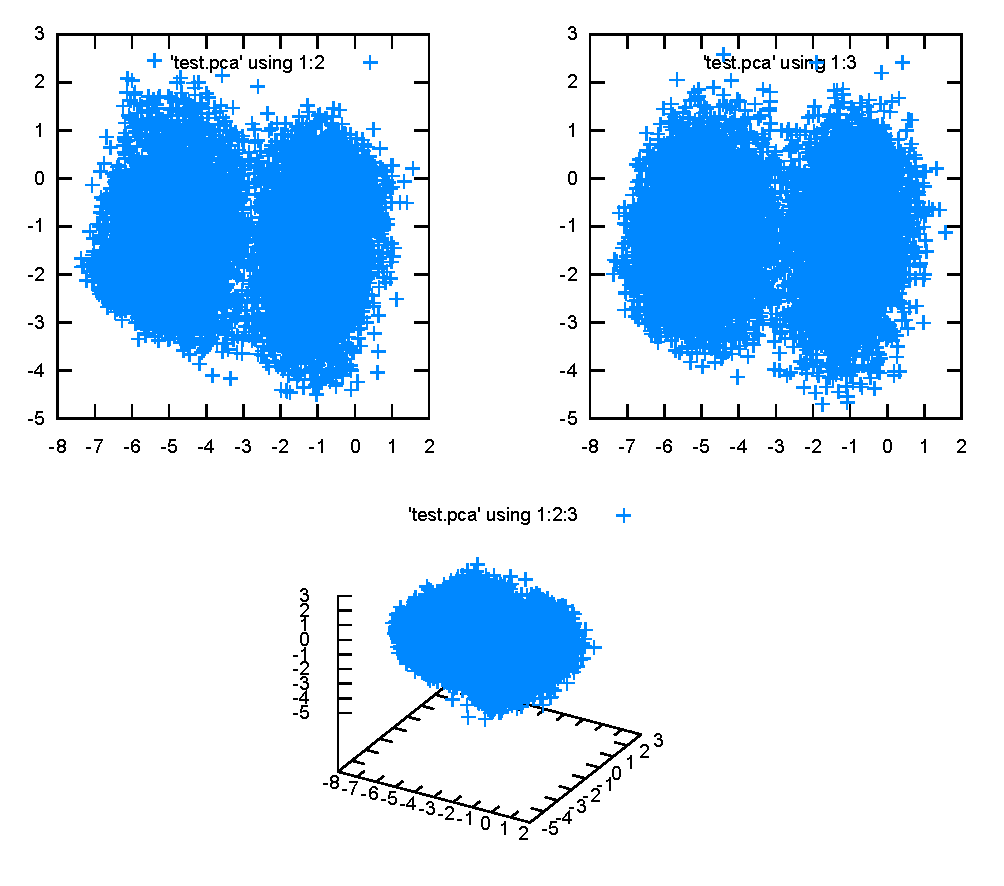
\includegraphics[scale=0.9]{pca-tutorial.pdf}
    \caption{Example plots of PCA projections, upper left composants 1
      and 2, upper right 1 and 3 and lower 1,2 and 3}
    \label{fig-pca-tutorial}
  \end{center}
\end{figure}
As outlined by the figure it might not be evident to detect
different clusters ( in this case 2 as the projection shows a dataset
like the one generated with the command shown in listing
\ref{lst-virtev-tutorial} ). For a deeper inspection you might refere
to the \emph{pca2densityfile} and \emph{pca2densitymap} tools shown in
sections \ref{sec-pca2densityfile} and \ref{sec-pca2densitymap}
respectivly. Besides this tool we further have a PCA sequence selector,
that allows us to extract and investigate sequences, from
dense ensembles, in literature also cited as comets \cite{lauriane},
and directly access the sequences. This tool is highlighted in section
\ref{sec-pcavisual}.

\section{Adaptive Clustering}

One core feature of the \emph{MNHN-Tools} is an adaptive density
based clustering algorithm that can be used to study phylogenetic
features and the evolution of species by investigating typical
DNA barcoding targets such as the 16S or 18S ribosomal RNA or
Cyclooxygenase 1 (COX1) coding regions. Further the tool might be of
use for all kinds of purposes where similar sequence clusters are to
be investigated. As such \emph{MNHN-Tools}
was successfully applied in the quest to discover families of
α-satellites, repeated sequences, in the human genome.

Adaptive clustering is implemented in the MNHN tools with different underlying
sequence distance measures and optimized for different computing
architectures. As we have already highlighted the PCA tools during the
tutorial and for the sake of the rapidity of the computation we show
how we can use the PCA based adaptive clustering method in order to
investigate our dataset of sequences:
\lstset{language=bash,
  caption={Performing PCA based adaptive clustering},
  label=lst-adaptivecluster-tutorial}
\begin{lstlisting}
mkdir clusters
adaptive_clustering_PCA test.fasta 1 0.001 3 clusters/L 2 7 test.pca > cl-out
\end{lstlisting}
Here we iterativly use the DBSCAN algorithm \cite{dbscan} from a
starting value of $\epsilon_{\mathrm{int}} = 1$ and increasing in it
each step by $\Delta\epsilon = 0.001$. Togther with the constant
\emph{minPoints} of 3 value this forms different density limits. The
scanning algorithm will find us sequences above these density limits,
and as the density decreases in each step regions that house connected
sequences above a certain density are growing and will merge, and
hence, denser regions are found to be in less denser regions. This
denser regions in less denser regions allow us the interpret
dependencies, build dendograms and investigate evolution. A simple
illustration of the algorithm is shown in figure
\ref{fig-adaptive-cluster}.
\begin{figure}
  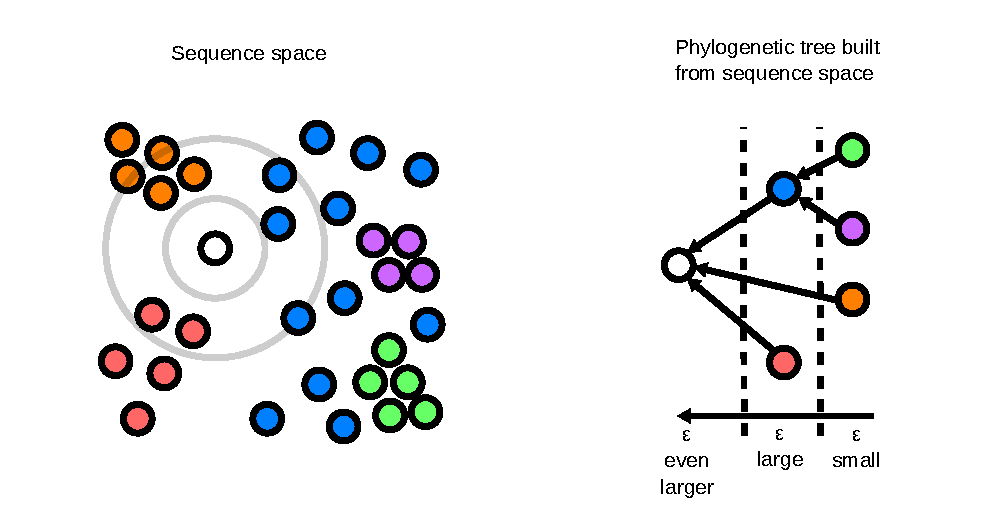
\includegraphics{densities-space.pdf}
  \caption{The adaptive clustering algorithm finds dense (new)
    clusters in less dense (old) more dispersed clusters. Finally the
    \emph{MNHN-Tools} collection allows us to build a tree from like
    the one on the right, from a sequence space as the one on the
    left.}
  \label{fig-adaptive-cluster}
\end{figure}
For a more detailed overview the reader is refered to section
\ref{sec-adaptive-clust}. 
The command in listing \ref{lst-adaptivecluster-tutorial} yields us
with an output file \emph{cl-out} and a bunch of binary
\emph{split-sets} in the
\emph{cluster} folder. A binary \emph{split-set} is a file that holds
a partitioning of our dataset. As we have run an adaptive clustering
run, serveral different partitions for different densities have been
returned by the algorithm. These will later on be the layers of our
tree. Hence we named them L, and the tool returned us files that hold
the name like \emph{L0000}, \emph{L0001} etc. indicating the layer of
the tree. From the most outer leaf node \emph{L0000} to the most inner
root \emph{LNNNN} with \emph{NNNN} being the highest number
available. For each of the clusterings we also know, thanks to the
data that we stored in \emph{cl-out} which binary \emph{split-set}
belongs to which $\epsilon$ and hence to which density limit.

\section{Tree Building, Tree Visualization and Tree Investigation}

Having our \emph{split-sets} from an adaptive clustering run at hand,
and having looked alread at the \emph{cl-out} file we already have
guessed what is next. In the \emph{cl-out} file different there is at
the lower and a list of connections between different clusters at
different layers. The next step is to build a tree, or a dendogram
representing the density structure of our dataset and hence obtain the
left side of figure \ref{fig-adaptive-cluster}. \emph{MNHN-Tools} comes
with a tool to infer a Newick tree \cite{newick} from the clusters
obtained during an adaptive clustering run. Here we run the tool
\emph{split\_sets\_to\_newick} outlined in section \ref{sec-ssnewick}
using the results from our adaptive clustering run:
\lstset{language=bash,
  caption={Generating a Newick tree with \emph{split\_sets\_to\_newick}},
  label=lst-ssnewick-tutorial}
\begin{lstlisting}
split_sets_to_newick 0 0 clusters/L* > tree.dnd
\end{lstlisting}
and obtain a Newick tree in the file \emph{tree.dnd}. You can use a
tool of choice to plot the Newick tree, but herein we show how to do
it with the Newick tools by the University of Geneva
\cite{newick_tools}.
\lstset{language=bash,
  caption={Using the Newick tools \cite{newick_tools} to plot a
    dendogram},
  label=lst-newick-tools-tutorial}
\begin{lstlisting}
nw_display -s -b 'opacity:0' -w 600 tree.dnd > tree.svg
\end{lstlisting}
where the options are \emph{-s} in order to generate a \emph{scalable
vector graphics} (SVG) file, \emph{-b 'opacity:0'} is here to hide the
number indicating the distance between the clusters. \emph{-w} the
size, with of the image. The reader shall be refered to the Newick
tools manual for all the vast possibilities of options. If you use
your own dataset you might have to adjust the width so that all the
labels are visible. In general you should be presented with a tree
like the one shown in figure \ref{fig-nwtree-tutorial}.
\begin{figure}
  \begin{center}
    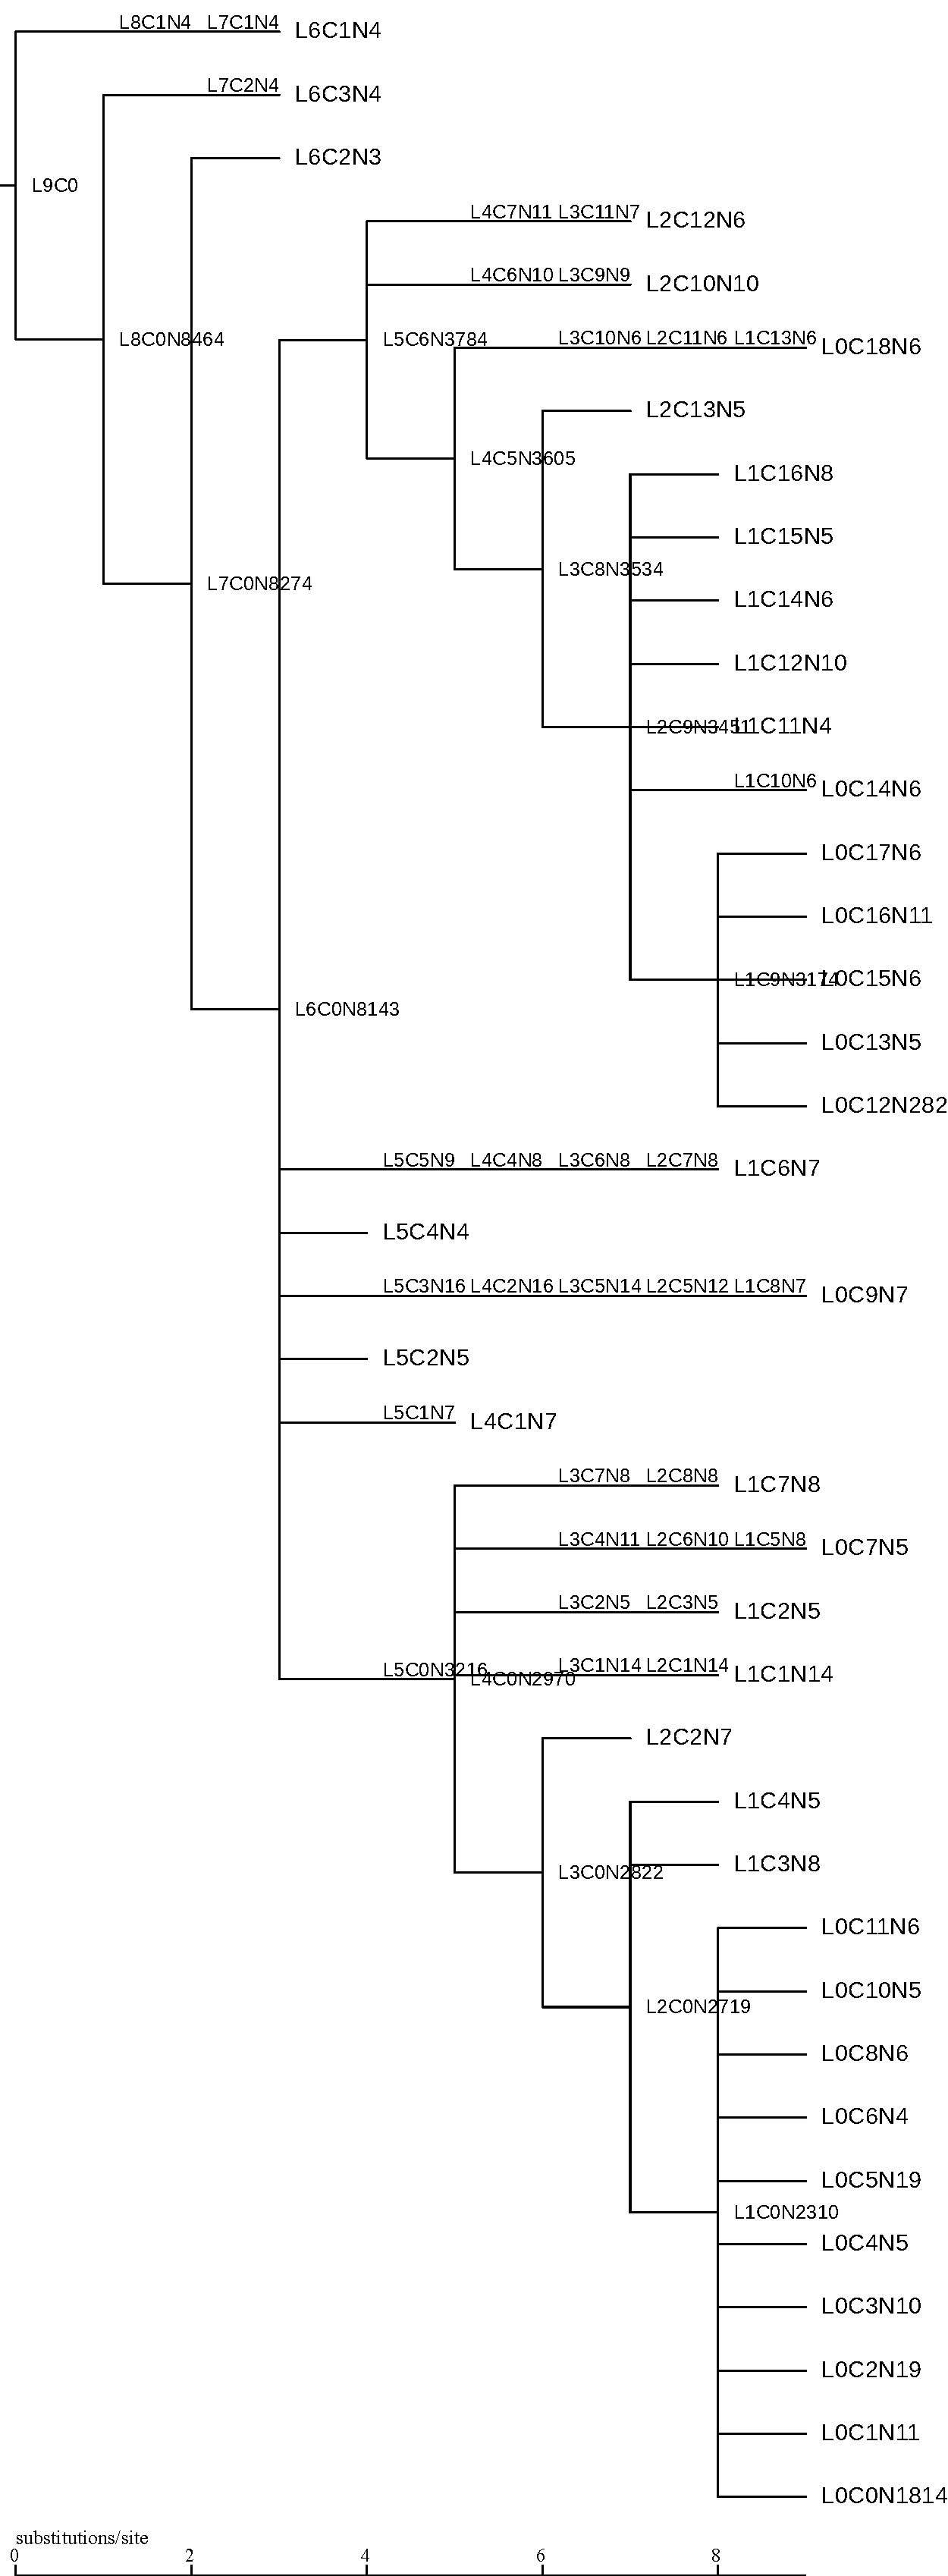
\includegraphics[scale=0.3]{nw-tree-tutorial.pdf}
    \caption{A Newick tree with the cluster labels visible, each
      cluster is labeld by L$X$C$Y$N$Z$ where $X$ is the layer number,
      $Y$ the cluster number and $Z$ the number of sequences in that
      cluster. The substitutions/site are automatically added by the
      Newick tools and have in our case no significance.}
    \label{fig-nwtree-tutorial}
  \end{center}
\end{figure}
Here in the image which is the tree of clusters obtained from our
virtual biophere, generated by the command in listing
\ref{lst-virtev-tutorial} where two partitions with a distance of at
least 5 nucleotides was requested. One of these underwent 10000 single
nucleotide mutations and the other 20000, and hence both partitions
diffused, as seen in the figures of the PCA \ref{fig-pca-tutorial} and as it
can be seen in the figures of the tree \ref{fig-nwtree-tutorial}.

Looking at figure \ref{fig-nwtree-tutorial}
Lets say we would like to identify the clustrs \emph{L5C0} containing
3216 sequences and \emph{L5C6} containing 3784 clusters. Both at the
forefront of two large subtrees. In order to acces the sequences in
these clusters we have to convert layer 5 to FASTA files. Layer 5
exists by \emph{MNHN-Tools} convention in a binary \emph{split-set}
file named with the suffix number \emph{0005}, hence in our case, as
demanded by the command in listing \ref{lst-adaptivecluster-tutorial}
named in the folder \emph{clusters} named \emph{L0005}. In order to
convert the sequences of layer 5 to \emph{FASTA} files we use the
tool \emph{split\_set\_to\_fasta} as described in section
\ref{sec-sstofasta}. We note here to the reader, that his personal tree, even
using our commands might slightly differ due to different random
number generater mechanisms on different systems, and that he might
have to adapt cluster and layer numbers to the tree he has obtained. 
The \emph{split\_set\_to\_fasta} tool is called here like:
\lstset{language=bash,
  caption={Converting a binary \emph{split-set} to \emph{FASTA} sequences},
  label=lst-sstofasta-tutorial}
\begin{lstlisting}
mkdir fasta-layer-5
split_set_to_fasta test.fasta clusters/L0005 fasta-layer-5/C
\end{lstlisting}
and hence we obtain the FASTA files for layer 5. The files foru our
clusters \emph{L5C0} and \emph{L5C6} are respectivly stored in the
files \emph{fasta-layer-5/C-000} and \emph{fasta-layer-5/C-006} in
FASTA format. Using the same mechanism we can identify any sequence
anywhere in the tree. Now one could open these files for instance with
\emph{SEAVIEW} and throw all kind of statistical tools, or our
\emph{consens} tool highlighted in section \ref{sec-consens} on this
files.

But let us do something more interesting let us identify the
two clusters in our PCA diagram, such as the one shown in figure
\ref{fig-pca-tutorial}. In order to do this we can use a tool called
\emph{split\_set\_to\_projections}, further described in section
\ref{sec-ssproj}. We run this tool likewise:
\lstset{language=bash,
  caption={Converting a binary \emph{split-set} to PCA projections},
  label=lst-ssproj-tutorial}
\begin{lstlisting}
mkdir projections-layer-5
split_set_to_projections test.fasta test.pca 7 clusters/L0005 \
  projections-layer-5/p
\end{lstlisting}
Analogus to the FASTA files we optain the files containing the PCA
projections of these clusters. Again in our case the projections for
\emph{L5C0} and \emph{L5C6} reside in files \emph{p-000} and
\emph{p-006} in folder \emph{projections-layer-5}. We can right now
use the \emph{gnuplot} \cite{gnuplot} software to locate them:
\lstset{language={},
  caption={Highlighting cluster projections with \emph{gnuplot}},
  label=lst-gnuplot-proj-tutorial}
\begin{lstlisting}
plot 'test.pca' using 1:2 lt rgb '#333333', \
'projections-layer-5/p-000' using 1:2 lt rgb '#FF8800', \
'projections-layer-5/p-006' using 1:2 lt rgb '#0088FF'
\end{lstlisting}
which generates in our case the figure \ref{fig-pca-proj}.
\begin{figure}
  \begin{center}
    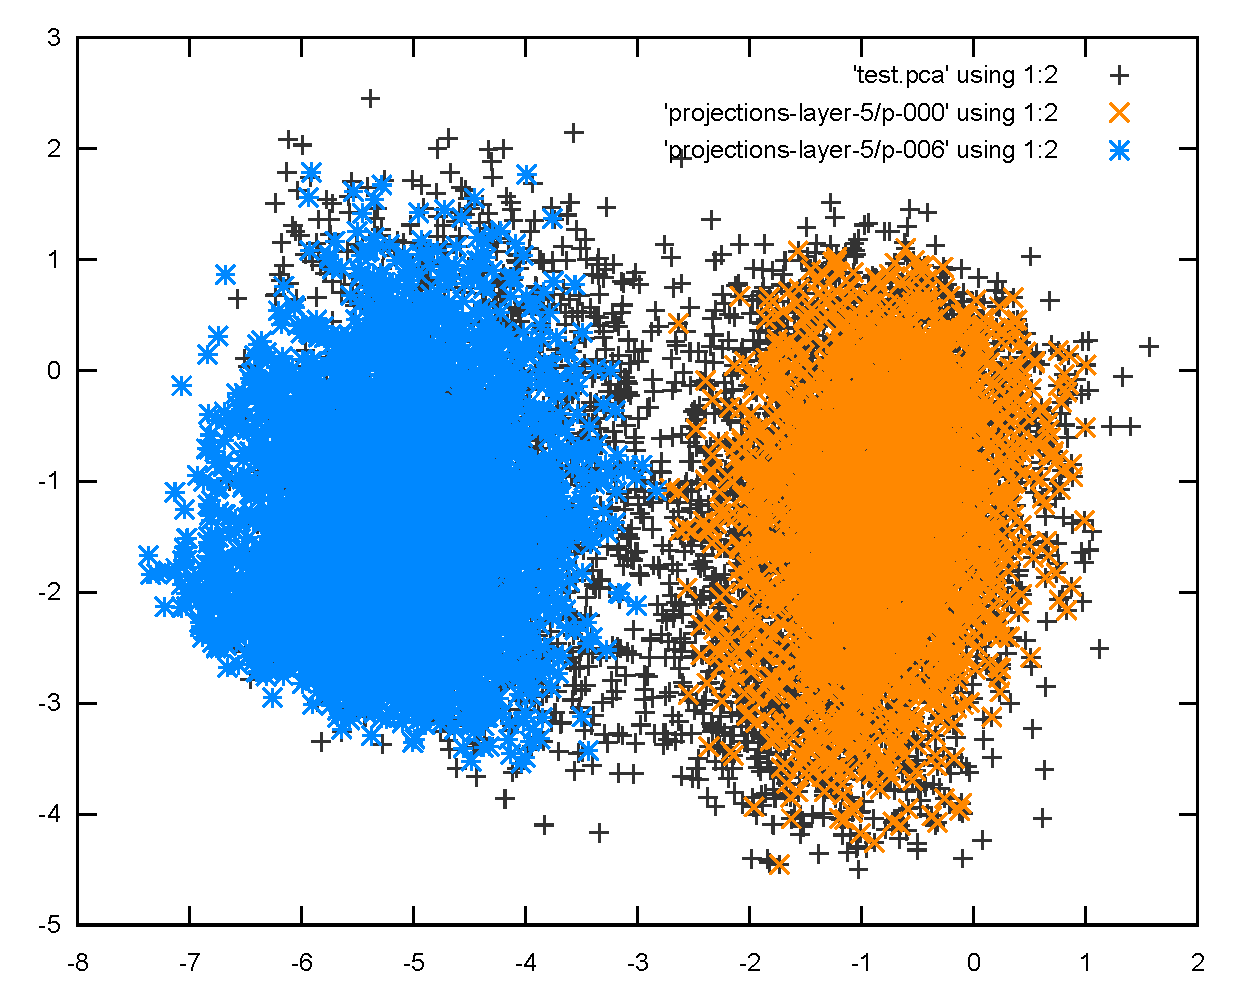
\includegraphics[scale=0.6]{pca-projections.pdf}
    \caption{The projections of cluster \emph{L5C0} in orange, and the
      projections of cluster \emph{L5C6} in blue projected onto the
      first two principal components}
    \label{fig-pca-proj}
  \end{center}
\end{figure}
Note that as the algorithm is written in order to infer the tree
structre and consensus ( center of gravity ) of clusters / sequence
families, sometimes the clusters might appear small when projected. In
this case you can search for a more optimal cluster size varing the
$\epsilon$ value around the layer in question. You can find this value
in the output file, in our case \emph{cl-out} as requested in listing
\ref{lst-adaptivecluster-tutorial}. You may find lines like the
following:
\lstset{language={},
  caption={Layer 5 description in our adaptive cluster run output
    file},
  label=lst-cl5-out-tutorial}
\begin{lstlisting}
Layer 5 has 7 clusters
  Coverage at layer 5: 0.704100
  Epsilon at layer 5: 1.100000
\end{lstlisting}
As the algorithm is tree preserving. If you have the feeling that the
clusters are to small you can run a single \emph{DBSCAN} run
\cite{dbscan} with the tools \emph{cluster\_dbscan\_X} tools
shown in section \ref{sec-dbscan-cluster},
choosing an epsilon value just below the one of the following layer,
which in this case is described to be:
\lstset{language={},
  caption={Layer 6 description in our adaptive cluster run output
    file},
  label=lst-cl6-out-tutorial}
\begin{lstlisting}
Layer 6 has 4 clusters
  Coverage at layer 6: 0.815400
  Epsilon at layer 6: 1.180000
\end{lstlisting}
This way more defuse sequences might be taken into account, just
before the clusters merge due to the $\epsilon=1.18$ density
critera. You can hence if you like oversample the tree.

Let us further investigate the structure of the tree, and let us say
we would like to see how a single sequence flows through the tree,
and where it appears in the tree. In order to achieve such a task we
have the \emph{three\_map\_for\_sequence} tool shown in section
\ref{sec-treemapseq}. Lets say we are interesed to find the following
sequence that resides in our initial dataset in our tree:
\lstset{language={},
  caption={A sequence of interest},
  label=lst-sequence-target-tutorial}
\begin{lstlisting}
>sequence_6773
CGGCTTACGAACTGCCGCTTGTTTCACCTGGGCACAGTGTACCACGCAAA
AGATGGAGTTACTCGCGGACAAATAGGGAGCGTTGTGTCCGGTGAGTTAG
\end{lstlisting}
We hence save this sequence into a separated FASTA file called
\emph{target.fasta}.
We can now use the the \emph{tree\_map\_for\_sequence} tool to create
a map for the Newick tools by issuing the following command:
\lstset{language=bash,
  caption={Mapping the \emph{target.fasta} sequence in the Newick tree},
  label=lst-treemapseq-tutorial}
\begin{lstlisting}
tree_map_for_sequence target.fasta test.fasta '#FF8800' clusters/L* > target.map
\end{lstlisting}
This allows us to color the clusters in the tree that contains the
target sequence. To generate a SVG file you can use the Newick tools
command:
\lstset{language=bash,
  caption={Drawing the dendogram highlighting the sequence in \emph{target.fasta}},
  label=lst-nwtools-highlight-seq-tutorial}
\begin{lstlisting}
nw_display -s -b 'opacity:0' -w 600 tree.dnd -c target.map > tree-seq6773.svg
\end{lstlisting}
which results in a dendogram as shown in figure \ref{fig-treemapseq-tutorial}.
\begin{figure}
  \begin{center}
    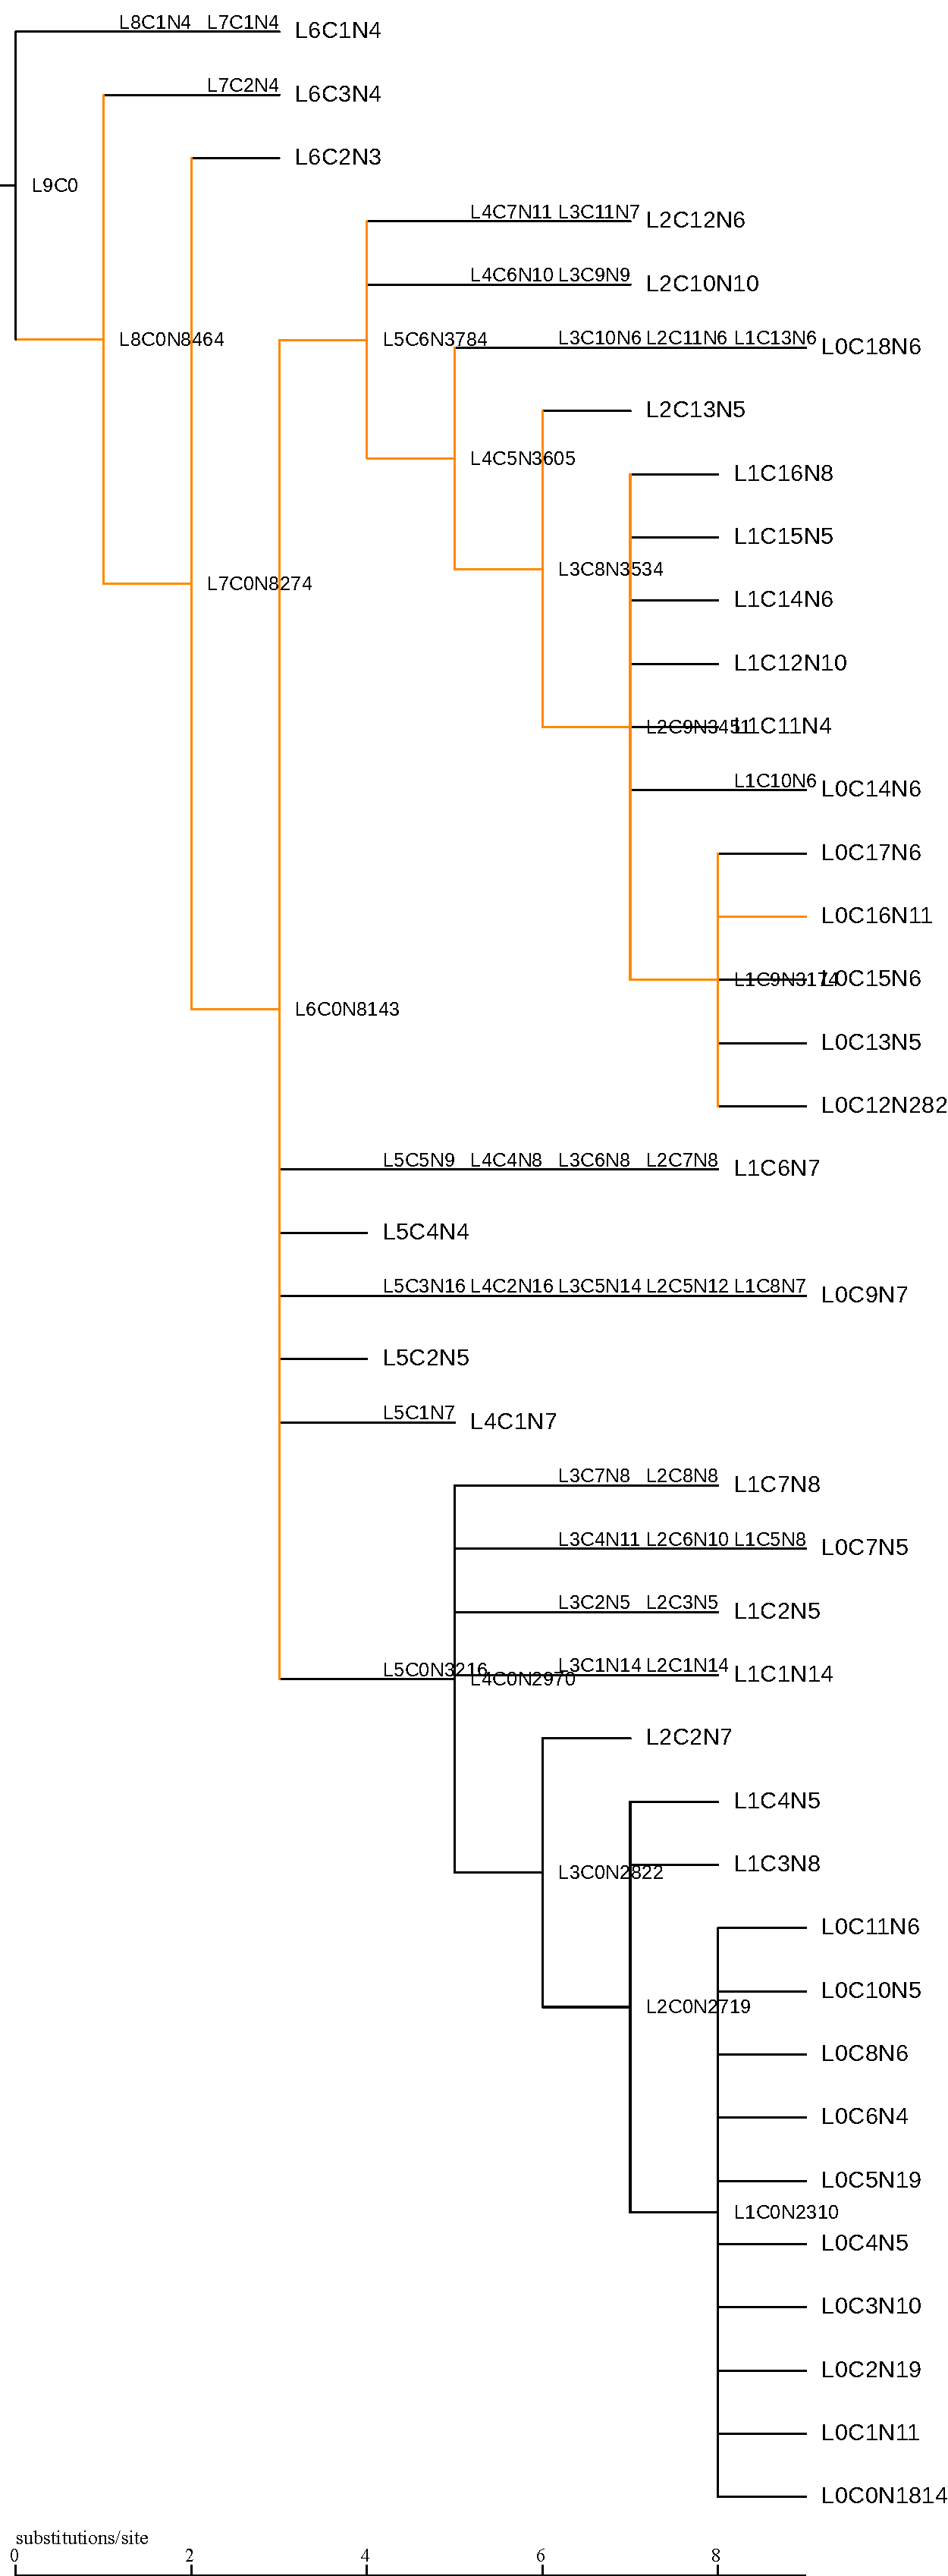
\includegraphics[scale=0.3]{nw-tree-sequence.pdf}
    \caption{The tree, tracing down a target sequence highlighted by
      the \emph{tree\_map\_for\_sequence} tool.}
    \label{fig-treemapseq-tutorial}
  \end{center}
\end{figure}

\section{Comparison to Ground Truth}

In this section we show you how you can investigate not just the location
of one single sequences but of a whole ensemble of sequences within the tree
obtained by an adaptive clustering run. If you know about certain
sequences that form a group in your own dataset you can follow us on
this route, generating your own clusters that you might want to
investigate in your own trees. The dataset generated with the command
highlighted in listing \ref{lst-virtev-tutorial} is partitioned as we
could also suggetst from the tree into two subgroups. The
\emph{virtual\_evolution} (c.f. section \ref{sec-virtual-ev}) tool has
generated two partitions of 5000 sequences. As the partitions are
written out sequencial by the \emph{virtual\_evolution} tool the
first 5000 sequences belong to the first partition, the next 5000
sequences belong to the second partition. We can thus generate an
artificial clustering or binary \emph{split-set} in order to further
investigate the two known partitions with the \emph{MNHN-Tools}. In
order to generate such a \emph{split-set} we will use the
\emph{split\_set\_from\_annotation} tool outlined in section
\ref{sec-ssannotation}. In order to do this with first have to
generate the annotation file. On the \emph{bash} \cite{bash} shell on
a Unix/Linux system you can do this in the following way:
\lstset{language=bash,
  caption={Generationg an annotation file for
    \emph{split\_set\_from\_annotation}},
  label=lst-ssannotation-annotation-tutorial}
\begin{lstlisting}
for ((i=0;i<5000;i++)); do echo "one" >> gt-annotation; done
for ((i=0;i<5000;i++)); do echo "two" >> gt-annotation; done
echo "one" >> unique-gt-annotation
echo "two" >> unique-gt-annotation
\end{lstlisting}
which creates us the \emph{gt-annotation} file that contains 5000
lines with just the single word \emph{one} on each line followed by an
other 5000 lines with the single word \emph{two} on each line. We
further create the \emph{unique-gt-annotation} file containing just
two lines with the statements \emph{one} and \emph{two}. The
\emph{unique-gt-annotation} file is used, first to describe that
statements that indicate the clusters to be formed, in our case
\emph{one} and \emph{two} and second to order the clusters in the
resulting \emph{split-set} file. As \emph{one} fills the first line,
and \emph{two} the seconds in the \emph{unique-gt-annotation} file we
know that sequences marked as \emph{one} in the \emph{gt-annotation}
file will be part of the first clusters while those marked to be
\emph{two} will be part of the second cluster. With these files at
hand we can execute the \emph{split\_set\_from\_annotation} command:
\lstset{language=bash,
  caption={Creation of a \emph{split-set} cluster file by manual
    annotation},
  label=lst-ssannotation-execution-tutorial}
\begin{lstlisting}
split_set_from_annotation test.fasta gt-annotation unique-gt-annotation \
  ground-truth
\end{lstlisting}
which generates us the ground truth binary \emph{split-set} indicating
the two clusters.

A question that one might ask, knowing that the first 5000 sequences
form a partition and the second 5000 sequences form an other partition
as created by using our \emph{virtual\_evolution} tools: Where are we
going to find these sequences in the tree. In order to investigate
such a matter we can use the \emph{tree\_map\_for\_split\_set} tool
as shown in section \ref{sec-treemapss}:
\lstset{language=bash,
  caption={Creating a Newick tools \cite{newick_tools} map file for a
    \emph{split-set}},
  label=lst-treemapss-tutorial}
\begin{lstlisting}
tree_map_for_split_set ground-truth test.fasta 1 2 '1,#000000' \
  clusters/L* > tree-one.map
tree_map_for_split_set ground-truth test.fasta 1 2 '2,#000000' \
  clusters/L* > tree-two.map
\end{lstlisting}
which yields us the \emph{tree-maps} that we can use with the Newick
tools \cite{newick_tools} to highlight different the different
datasets in the trees. In order to do this we generate two SVG files
for each tree executing:
\lstset{language=bash,
  caption={Using the Newick tools \cite{newick_tools} to visualize
    partitions},
  label=lst-nwtools-highlight-ss-tutorial}
\begin{lstlisting}
nw_display -s -b 'opacity:0' -w 600 tree.dnd -c tree-one.map > tree-one.svg
nw_display -s -b 'opacity:0' -w 600 tree.dnd -c tree-two.map > tree-two.svg
\end{lstlisting}
together with the dendogram created in listing \ref{lst-ssnewick-tutorial}.
The two resulting trees are shown in figure \ref{fig-treemapss-tutorial}.
\begin{figure}
  \begin{center}
    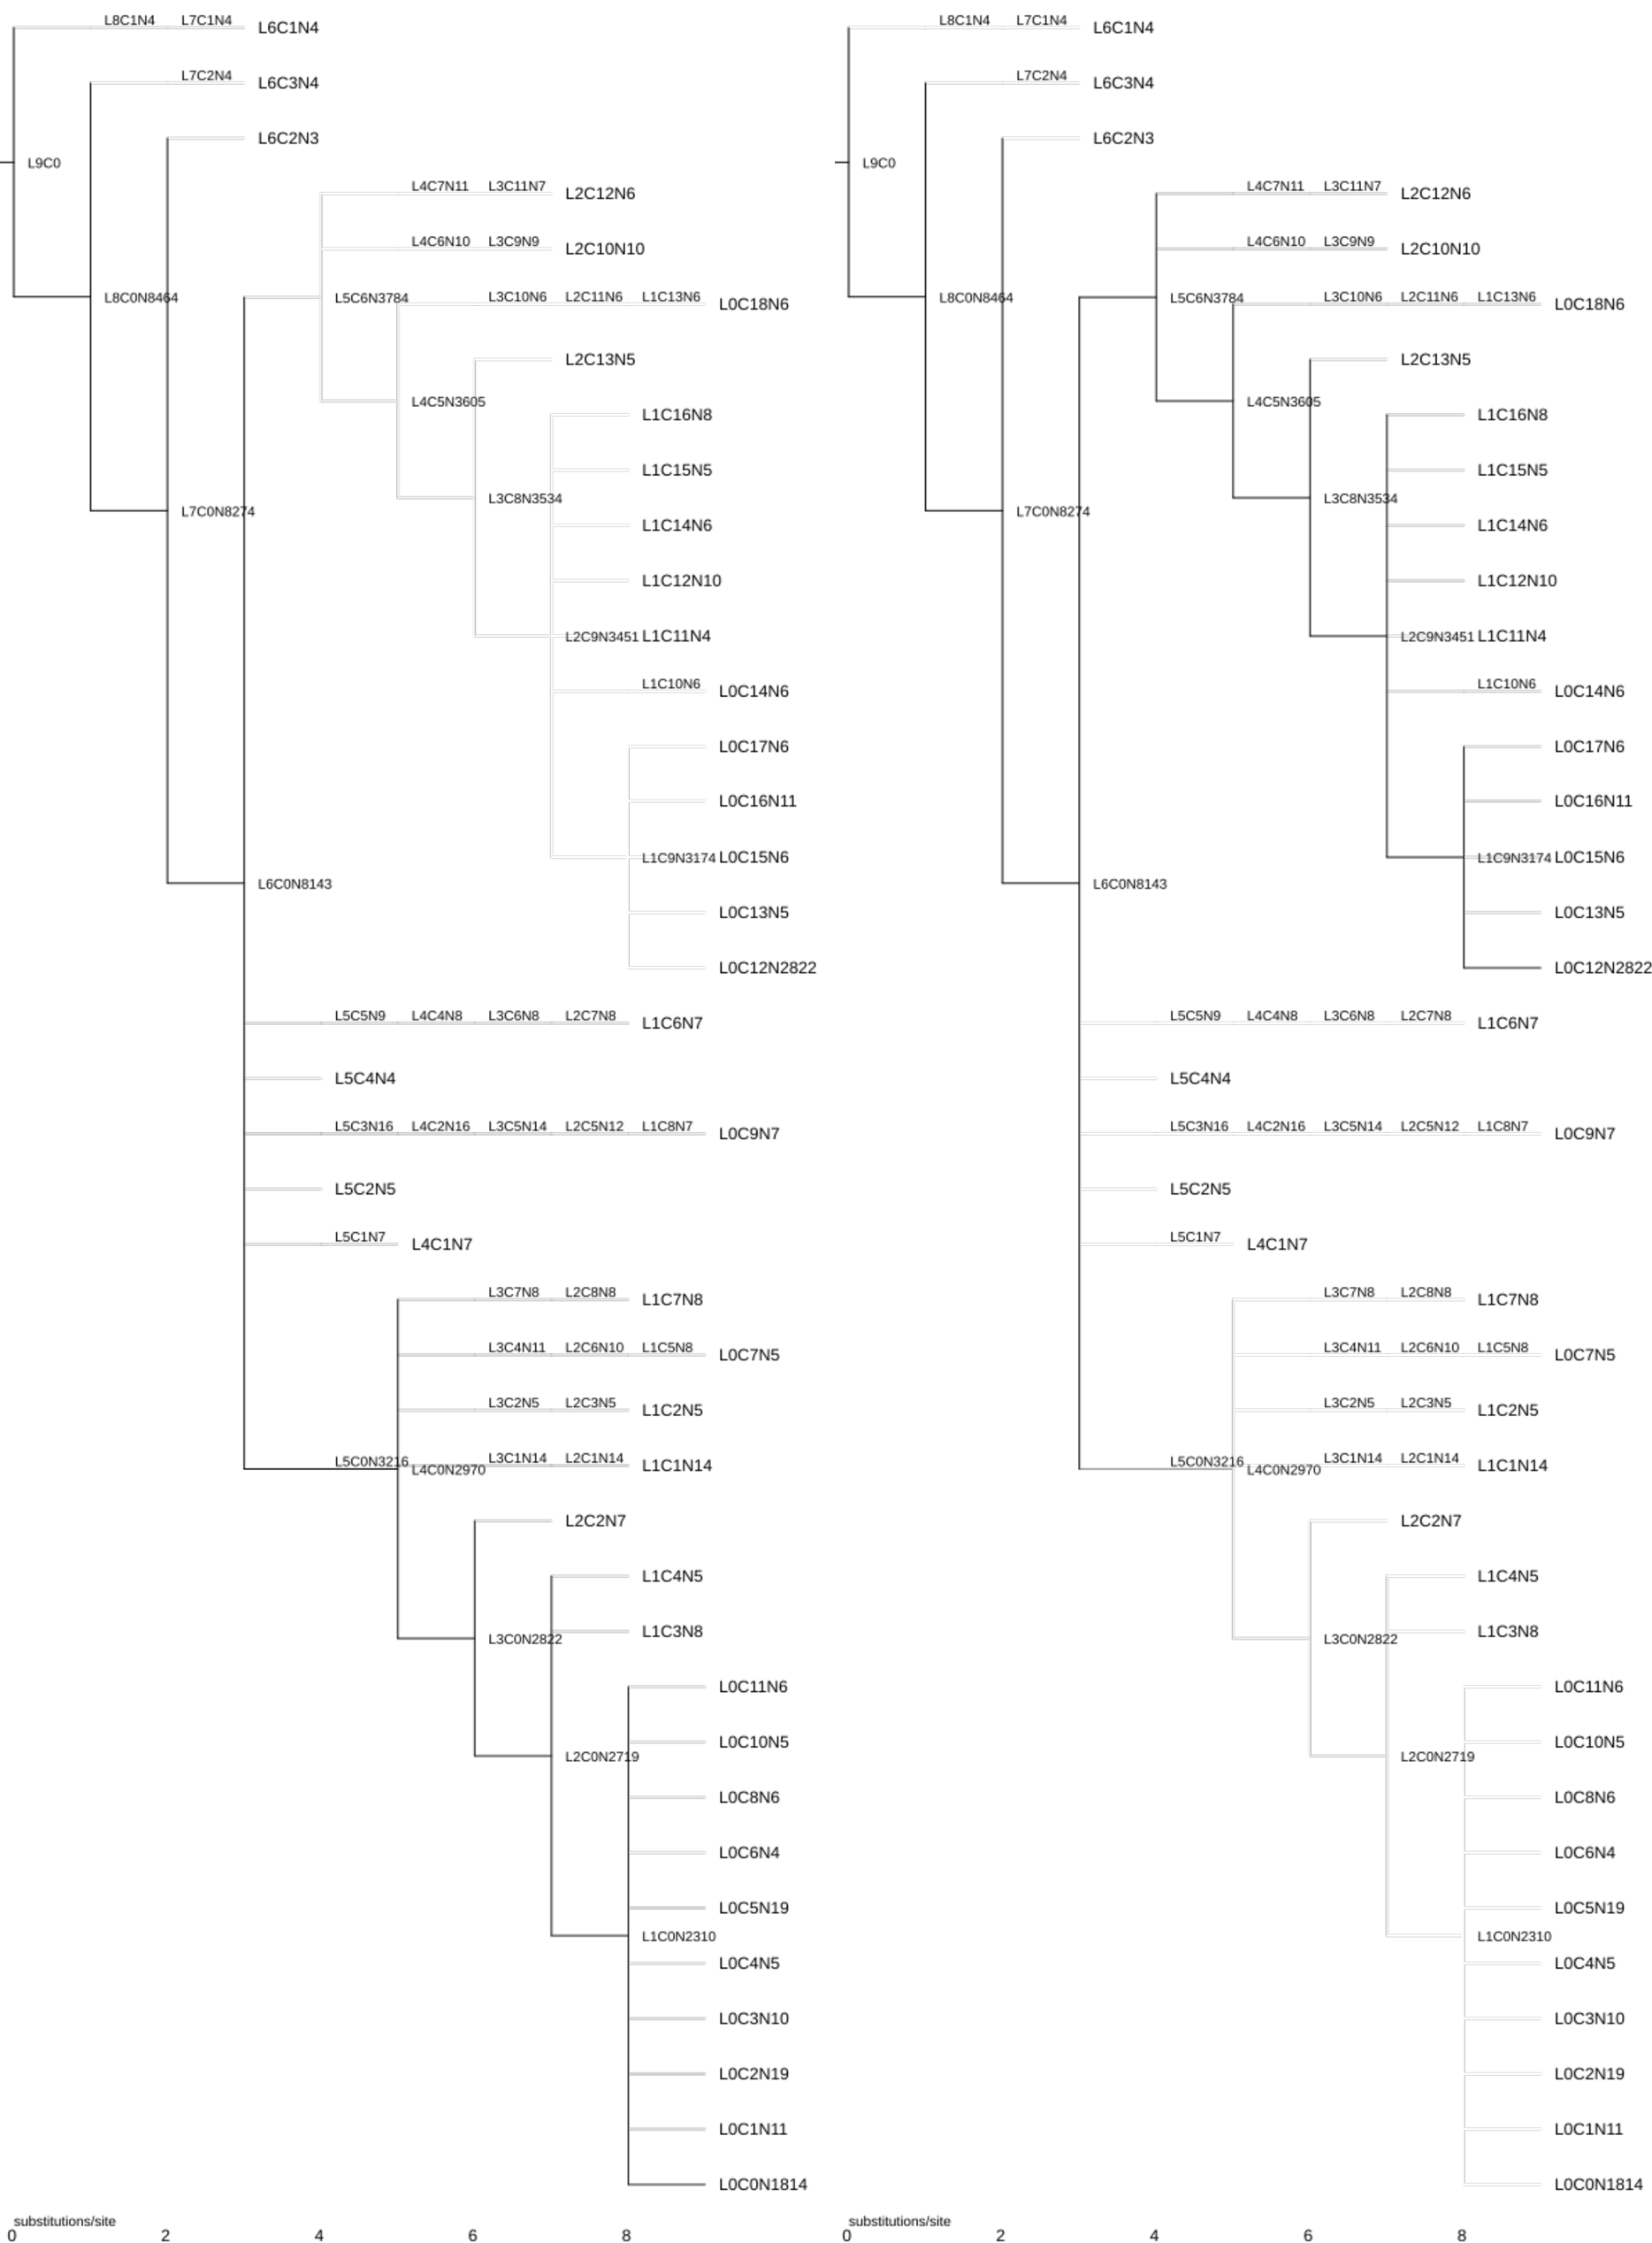
\includegraphics[scale=0.3]{tree-clust-tutorial.pdf}
    \caption{Tracing down clusters using the
      \emph{tree\_map\_for\_split\_set} tool. On the left we have the
      first partition while on the right the second partition is
      shown. Using the logarthmic representation we can also easily
      track down the core clusters \emph{L0C0} and \emph{L0C12} that
      have generated these two families, forming these two substrees
      (lower on the right, upper on the left).}
    \label{fig-treemapss-tutorial}
  \end{center}
\end{figure}
Finally we can quantize if our tree correctly maps the two
clusters by applying our \emph{Pureness} calculation. This allows us
to check weather we obtain the same clusters as the ground truth and
weather clusters are a mixture of the ground truth or not. For the
details of the Pureness, and other indices to evaluate the quality of
a tree against ground truth the reader is refered to section
\ref{sec-pureness}. In order to perform this quality measurement we
execture the \emph{tree\_pureness} tool:
\lstset{language=bash,
  caption={Evaluating a tree against ground truth with the
    \emph{tree\_pureness} Tool},
  label=lst-pureness-tutorial}
\begin{lstlisting}
tree_pureness test.fasta ground-truth clusters/L* > pureness
\end{lstlisting}
from where we obtain the following table:
\lstset{language={},
caption={The output of the \emph{Pureness} table},
label=lst-pureness-output-tutorial}
\begin{lstlisting}
0.001103        8.500000        0.052632
0.250433        7.500000        0.117647
0.134946        6.000000        0.214286
0.002904        5.000000        0.166667
0.002793        3.000000        0.250000
0.002923        2.500000        0.285714
0.978448        1.000000        0.500000
0.981508        0.500000        0.666667
0.969282        0.000000        0.500000
0.973321        0.500000        1.000000
\end{lstlisting}
where the first column is the Purness as in equation
\ref{eqn-pureness}, the second the Cluster Correspondance according to
equation \ref{eqn-c-corr} and finally the Impure over Pures as
outlined in equation \ref{eqn-impure-pure}. The table shows the values
for each layer from the leaf nodes on top to the root of the three on
the bottom. We see that in Layer 5 (we count from the top, and note
that the first line correponds to Layer 0)
we have a very good Pureness of 0.003 which counts only for the
already impure clusters, and that only about quater 28\% of the
clusters ( as shown in the third column ) are impure. The middle
column shows that at this moment the tree, nevertheless is not only
composed of two Datasets, but contains more clusters in this Layer. A
quick look at the Tree in figure \ref{fig-nwtree-tutorial} shows that
these clusters have very few elements and have formed due to the
fluctuation of diffusion. They would have been filtered away by a more
agressive \emph{minPoints} value in the adaptive clustering run.



